\documentclass[11pt]{article}
\usepackage{enumerate}
\usepackage[T1]{fontenc}
\usepackage[top=1in, bottom=1in, left=1.25in, right=1.25in]{geometry}
\usepackage{graphicx}
\newcommand{\itab}[1]{\hspace{0em}\rlap{#1}}
\newcommand{\tab}[1]{\hspace{1em}\rlap{#1}}
\title{Homework 3 for Intro to Computational Complextiy}
\author{Shenlong Gu}
\date{917-544-8927, sg3301@columbia.edu, 2, Nov 2015}
\begin{document}
\maketitle
\part{}

\def \vf {$V_{1}(x,c)$}
\def \vs {$V_{2}(x,c)$}
\def \v {$V(x,c)$}
\def \mf {$M_{1}$}
\def \ms {$M_{2}$}
\def \lf {$L_{1}$}
\def \ls {$L_{2}$}
    According to the definition of a strong nondeterministic turning machine, for a language $L$ belonging to SNTM, there is a $V(x, y)$, for each input
    $x$ $\in$ $L$, for all configuration path $y$, $V(x, y)$ will output "yes" or "maybe" and at lease one configuration path output "yes". For each input
    $x$ $\notin$ $L$, for all configuration path $y$, $V(x, y)$ will output "no" or "maybe" and at lease one configuration path output "no". \\ 
    First, we will prove $L$ $\in$ NP. \\
    We will construct a verification turning machine $V_{1}(x, y)$ by $V(x, y)$, just change the output "maybe" to "no". We can see for input $x$ $\in$ $L$, 
    at least one configuration path will output "yes", for $x$ $\notin$ $L$, all configuration paths will output "no". So $L$ $\in$ NP. \\ 
    Second, we will prove $\overline{L}$ $\in$ NP to prove $L$ $\in$ co-NP. \\
    We will construct a verification turning machine for $\overline{L}$, $V_{2}(x, y)$ by $V(x, y)$, just change the output "maybe" to "no", "yes" to "no", "no" to "yes". We can see for input $x$ $\in$ $\overline{L}$, at least one configuration will make $V(x,y)$ output "no", which means $V_{2}(x, y)$ will output "yes", and for $x$ $\notin$ $\overline(L)$, all configurations will make $V(x,y)$ output "yes" or "maybe" which means $V_{2}(x, y)$ will always output "no", so $\overline{L}$ $\in$ NP, $L$ $\in$ co-NP.
\part{}
    Because we know vertex cover problem is in NPC, we will reduce vertex cover problem to dominating set problem to prove dominating set problem is in NPC. \\
    Given a graph $G(V,E)$, we will construct a new graph $G'$, for each edge $e$, $(v_{i},v_{j})$, we add a new vertex $v_{k}$ and two edges, $(v_{k},v_{i})$ and $(v_{k},v_{j})$ and we get the new graph $G'$. (The reason why we do it is to change edge cover problem to vertex cover problem). \\
    We will then prove two problems are equivalent. First if there is a vertex cover with size $\leq$ $k$, obviously, these $k$ vertexes will form a dominating set, (the reason is that all edges is covered which means these $k$ nodes will sure connect to other nodes). Second, we will prove if there is a dominating sets with size $\leq$ $k$, then there is a vertex cover with nodes size $\leq$ $k$. We can see that we don't need to use the nodes newly added in graph $G'$, because we can easily replace $v_{k}$ by $v_{i}$ or $v_{j}$, then we can see if $k$ nodes which form the dominating sets will be the solution for vertex cover problem. Imagine, if there is an edge with two vertexes not in the dominating set, which means the corresponding vertex $v_{k}$ won't be connected by the dominating set and we get a contradictory so we can construct a vertex cover sets by the dominating set, so the dominating set problem belongs to NPC.
\part{}
    We will prove by reducing from the 3SAT problem. Because a graph is hard to draw, so I take a photo, as shown below: \\
    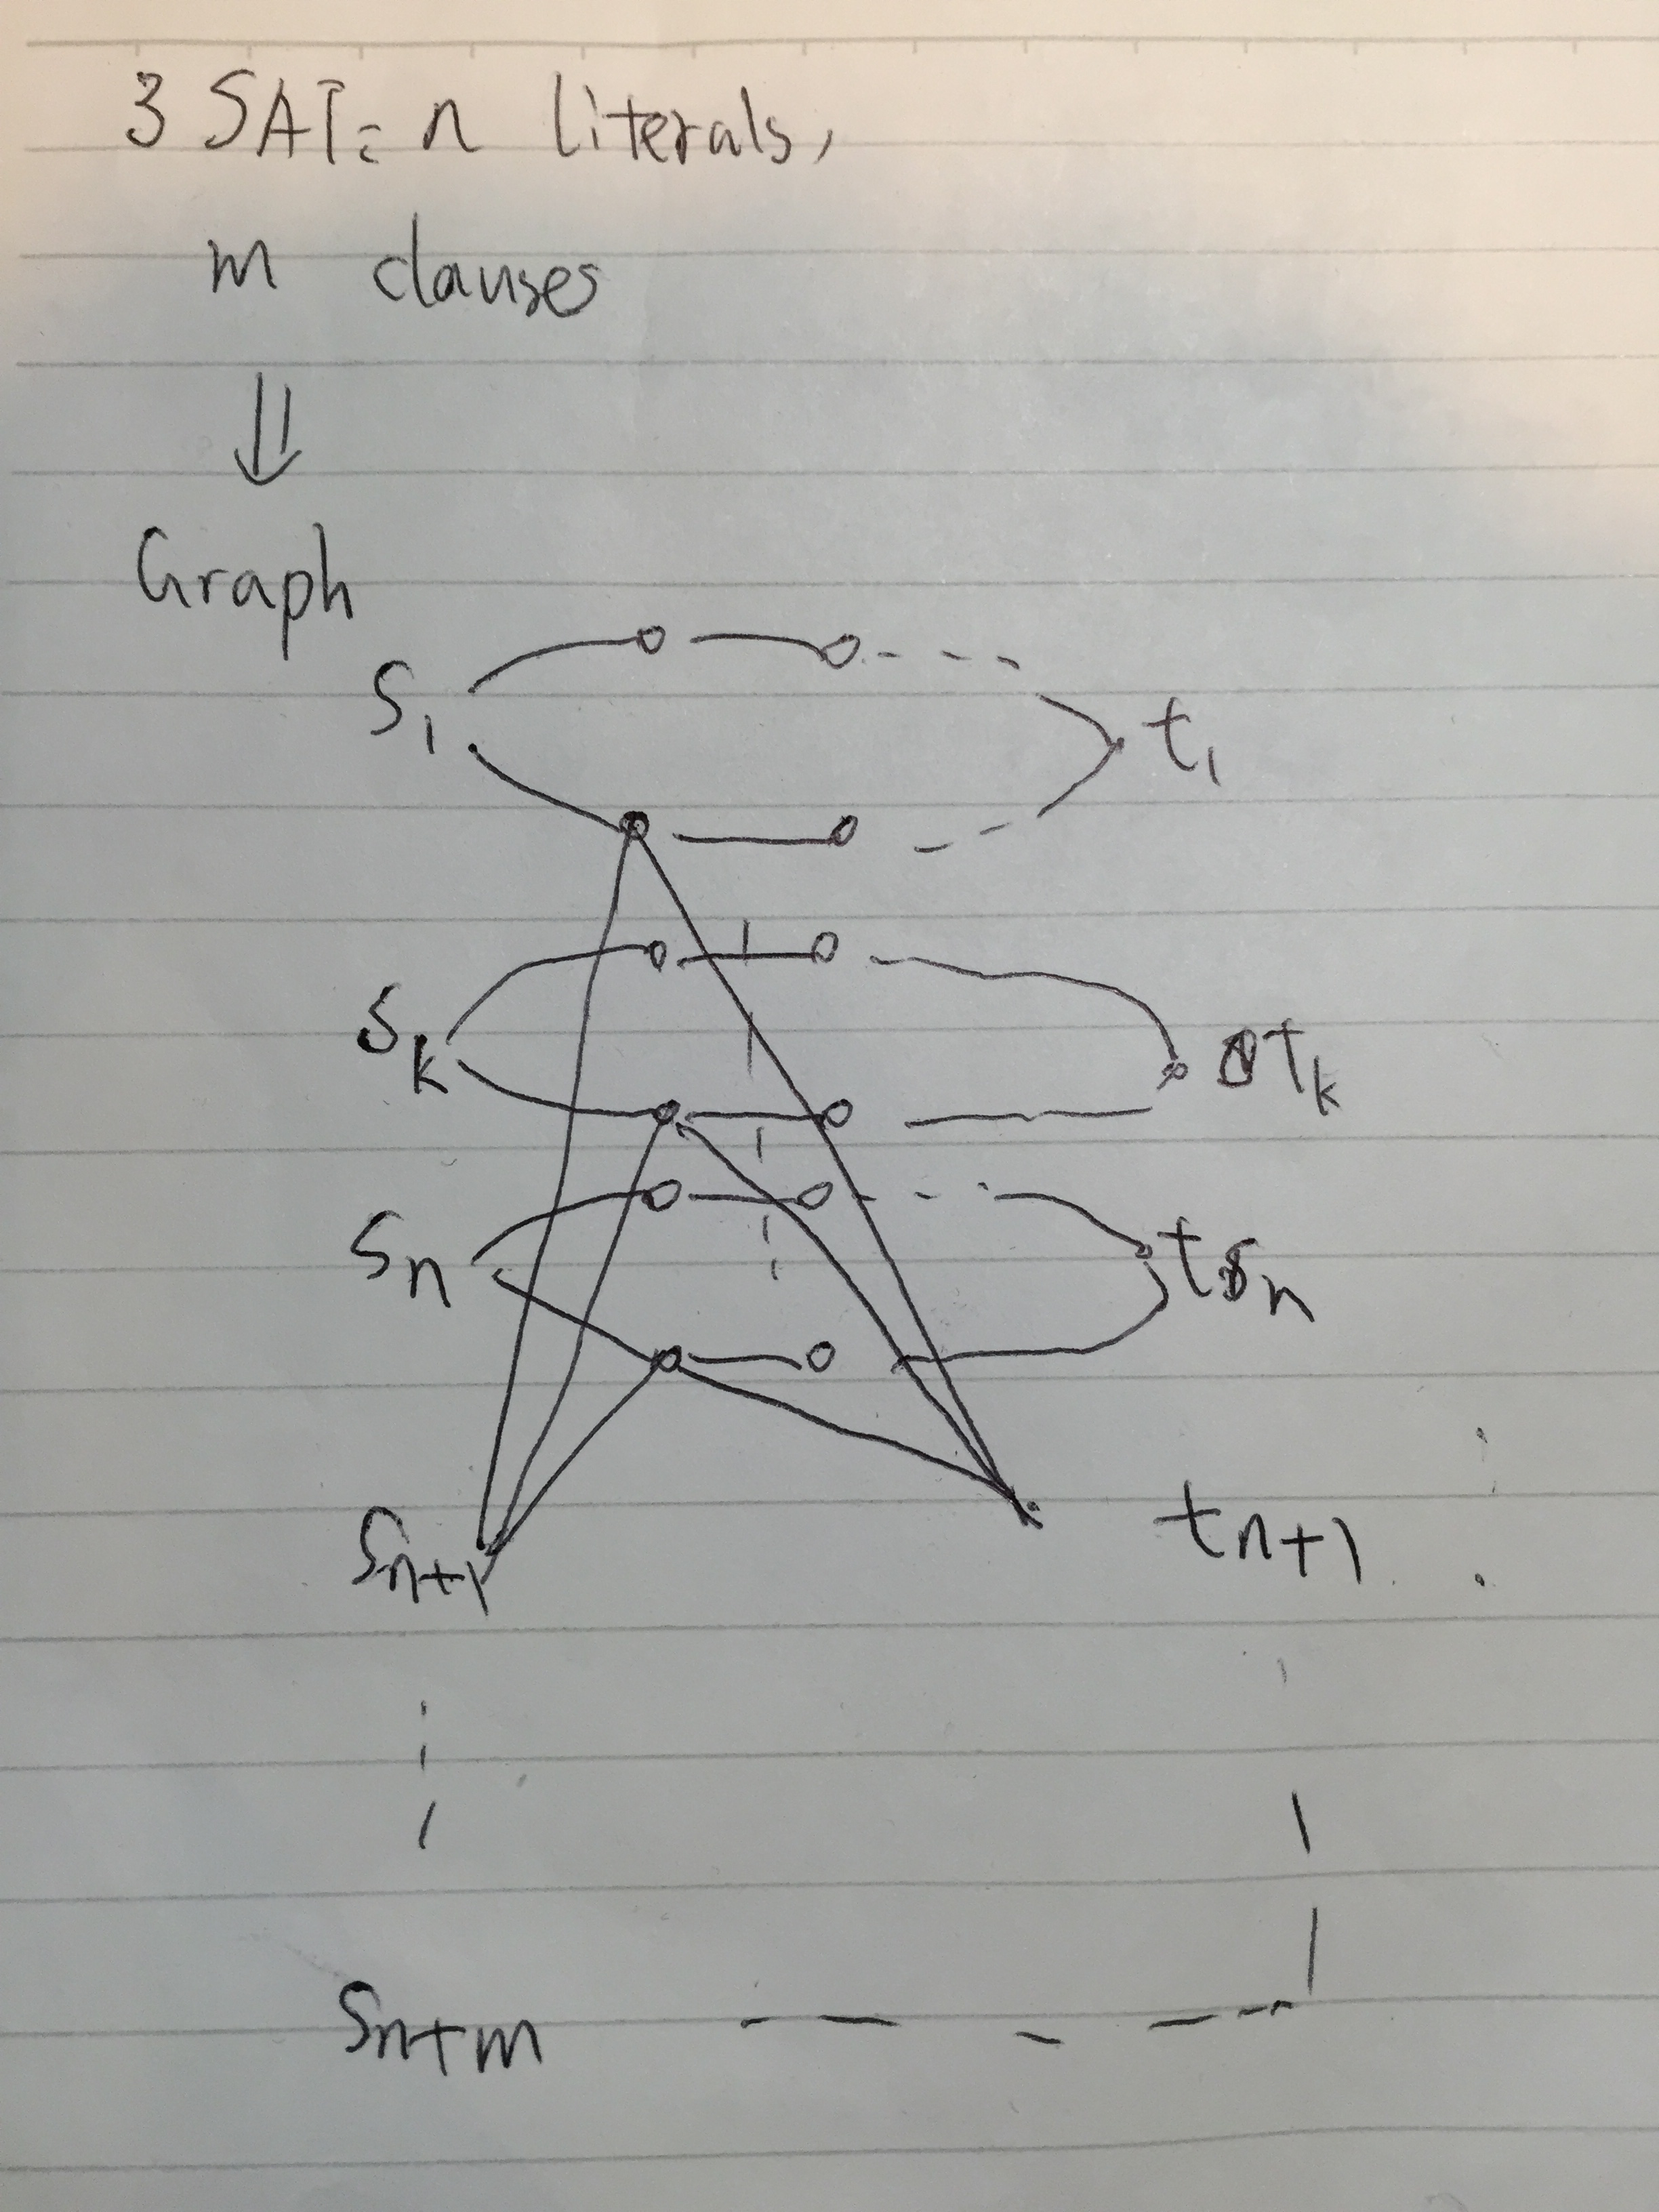
\includegraphics[width=5in]{part3}\\
    As shown in the photo, we map $n$ literals and $m$ clauses into $n+m$ paths. There are two paths for each variables for $s_{1}$..$s_{n}$ which represents true or false of each boolean variable. And there are three paths for each clauses, $s_{n+1}$..$s_{n+m}$. 
    The example shown in the photo is that the first clause is $\overline{x_{1}}$ $\cup$ $x_{k}$ $\cup$ $x_{n}$. We just construst the graph like this, we can see that for a clause takes a path, for example, $s_{n+1}$ takes the path from $s_{1}$..$t_{1}$, then $s_{1}$ will take the opposite path, otherwise there will be a node-joint. And if there is a assignment satisfying 3SAT, we can construct $n+m$ paths like this, and we can get an assignment satisfying 3SAT if there is $n+m$ paths with node-disjoint in the graph in return. So Disjoint Paths problem belongs to NPC.
\part{}
    To Be Solved
\part{}
    1. First, we look at the problem CLIQUE = {(G,k), there exists a clique of G has at least k vertices}. Because CLIQUE in NP, and P = NP, so CLIQUE in P. Then given a graph, $G$, we just enumerate $i$ from 1 to $n$ ($n$ is the number of nodes in the graph). And obviously there will be a $k_{1}$, for $i$ from 1 to $k$, CLIQUE with input $G$ and $i$ will output "yes" and for $i$ from $k_{1}+1$ to $n$ (if $k_{1}$ equals $n$, this interval will not exist), CLIQUE with input $G$ and $i$ will output "no". So we can compare $k_{1}$ with $k$ to see if this two number is equal. So we can see MAX-CLIQUE can be solved in P and it is easy to find the largest cliques. \\
    2. First, we will prove MAX-CLIQUE in $\Sigma_{2}^{P}$. 
        For input (G,k), $\exists$ a subset of nodes $y'$, and $\forall$ subsets of nodes $z'$, $V(x, y',z')$ = 1.
        $V(x, y',z')$ works as the follows: \\
        if the subset $y'$ doesn't form a clique of $k$, reject. \\
        if $z'$ form a clique larger than k, reject. \\
        Otherwise accept.\\
        So by definition of $V(x, y',z')$, we can see MAX-CLIQUE in $\Sigma_{2}^{P}$. \\
        Then, we will prove MAX-CLIQUE in $NP^{SAT}$. We can just nondeterministiclly select a subset $y'$, if $y'$ is not a clique of $k$, rejects, otherwise, because CLIQUE can be reduced to SAT, we can ask the oracle-SAT a question: whether if there is a clique of G has at least k+1 vertices. If the answer is yes, reject, otherwise accept. So MAX-CLIQUE in $NP^{SAT}$.
\part{}
    
\end{document}